
\begin{lstlisting}[language=Python,caption={Python function assignment example.}, label={lst:python-augment-twice-bad}]
def augment_twice_bad(a_list, val):
    """Put val on the end of 'a_list' twice."""
    a_list = a_list + [val, val]

nums = [1, 2, 3]
augment_twice_bad(nums, 4)
print(nums)             # [1, 2, 3]
\end{lstlisting}


When calling the function \texttt{augment\_twice\_bad}, the parameters are assigned the values \texttt{nums} and \texttt{4} respectively. 

\begin{center}
\texttt{augment\_twice\_bad(nums, 4)}
\end{center}

\begin{center}
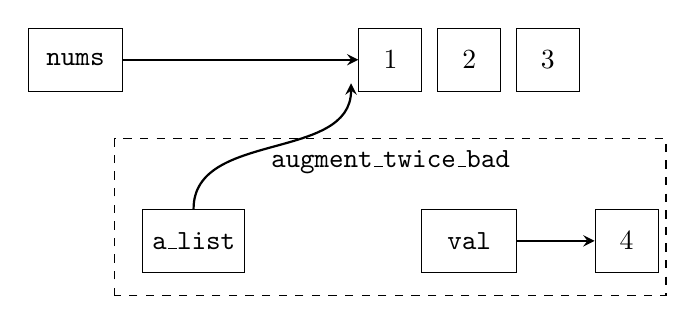
\begin{tikzpicture}[
    box/.style={rectangle, draw, minimum width=0.8cm, minimum height=0.8cm},
    varbox/.style={rectangle, draw, minimum width=1.2cm, minimum height=0.8cm},
    arrow/.style={->, >=stealth, thick}
]

% nums variable and list (outside function)
\node[varbox] (nums) at (-4, 1.5) {\texttt{nums}};
\node[box] (list1) at (0, 1.5) {1};
\node[box] (list2) at (1, 1.5) {2};
\node[box] (list3) at (2, 1.5) {3};

% Function frame (dashed rectangle)
\draw[dashed] (-3.5, -1.5) rectangle (3.5, 0.5);
\node at (0, 0.2) {\texttt{augment\_twice\_bad}};

% Function parameters
\node[varbox] (a_list) at (-2.5, -0.8) {\texttt{a\_list}};
\node[varbox] (val) at (1, -0.8) {\texttt{val}};
\node[box] (val_content) at (3, -0.8) {4};

% Arrows
\draw[arrow] (nums) -- (list1);
\draw[arrow] (a_list) to[out=90, in=270] (-0.5, 1.2);
\draw[arrow] (val) -- (val_content);

\end{tikzpicture}
\end{center}


The next statement is an assignment. The expression on the right-hand side makes a new list, which is then assigned to \texttt{a\_list} thus any further modification is made to the local variable only:

\begin{center}
\texttt{a\_list = a\_list + [val, val]}
\end{center}

\begin{center}
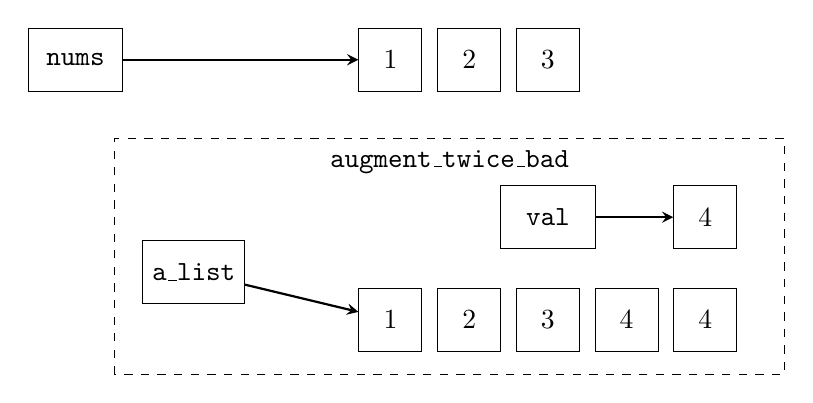
\begin{tikzpicture}[
    box/.style={rectangle, draw, minimum width=0.8cm, minimum height=0.8cm},
    varbox/.style={rectangle, draw, minimum width=1.2cm, minimum height=0.8cm},
    arrow/.style={->, >=stealth, thick}
]

% nums variable and original list (outside function)
\node[varbox] (nums) at (-4, 2.5) {\texttt{nums}};
\node[box] (orig1) at (0, 2.5) {1};
\node[box] (orig2) at (1, 2.5) {2};
\node[box] (orig3) at (2, 2.5) {3};

% Function frame (dashed rectangle)
\draw[dashed] (-3.5, -1.5) rectangle (5, 1.5);
\node at (0.75, 1.2) {\texttt{augment\_twice\_bad}};

% Function parameters
\node[varbox] (val) at (2, 0.5) {\texttt{val}};
\node[box] (val_content) at (4, 0.5) {4};

\node[varbox] (a_list) at (-2.5, -0.2) {\texttt{a\_list}};

% New list that a_list now points to
\node[box] (new1) at (0, -0.8) {1};
\node[box] (new2) at (1, -0.8) {2};
\node[box] (new3) at (2, -0.8) {3};
\node[box] (new4) at (3, -0.8) {4};
\node[box] (new5) at (4, -0.8) {4};

% Arrows
\draw[arrow] (nums) -- (orig1);
\draw[arrow] (a_list) -- (new1);
\draw[arrow] (val) -- (val_content);

\end{tikzpicture}
\end{center}

When the function ends, its local names are destroyed, and any values no longer referenced are reclaimed, leaving us just where we started:

\begin{center}
\texttt{print(nums)}
\end{center}

\begin{center}
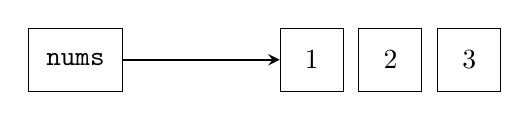
\begin{tikzpicture}[
    box/.style={rectangle, draw, minimum width=0.8cm, minimum height=0.8cm},
    varbox/.style={rectangle, draw, minimum width=1.2cm, minimum height=0.8cm},
    arrow/.style={->, >=stealth, thick}
]

% nums variable and list (back to original state)
\node[varbox] (nums) at (-2, 0) {\texttt{nums}};
\node[box] (list1) at (1, 0) {1};
\node[box] (list2) at (2, 0) {2};
\node[box] (list3) at (3, 0) {3};

% Arrow
\draw[arrow] (nums) -- (list1);

\end{tikzpicture}
\end{center}

If the goal was to modify the list passed in, the \texttt{=} operator can not be used. Instead, a method that mutates the list in place should be used, such as \texttt{list.append()} or \texttt{list.extend()}. The correct implementation of the function would be:

\begin{lstlisting}[language=Python, caption={Correct implementation of augment\_twice\_good}, label={lst:python-augment-twice-good}]
def augment_twice_good(a_list, val):
    """Put val on the end of 'a_list' twice."""
    a_list.extend([val, val]) # Mutates the list in place: [1, 2, 3, 4, 4]

# Or, an in-place addition:
def augment_twice_good(a_list, val):
    """Put val on the end of 'a_list' twice."""
    a_list += [val, val] # Mutates the list in place: [1, 2, 3, 4, 4]

\end{lstlisting}